\section{Renormalization Group Part II}
Today, we will go through the RG procedure on a model which is exactly solvable. 

\subsection{Exact Solution of Gaussian Model}
Consider the following partition function for a Gaussian model:
\begin{equation}
    Z = \int \mathcal{D}m(x)\exp\left(-\int d^dx \left(\frac{1}{2}tm^2 + \frac{1}{2}k(\nabla m)^2 + \frac{1}{2}L(\nabla^2 m)^2 - mh\right)\right)
\end{equation}
We go into momentum space:
\begin{equation}
    m(\v{q}) = \int d^dx e^{i\v{q} \cdot \v{x}}m(\v{x})
\end{equation}
Then:
\begin{equation}
    m(\v{x}) = \sum_{\v{q}}\frac{e^{-i\v{q} \cdot \v{x}}}{V}m(\v{q}) = \int \frac{d^d q}{(2\pi)^d}m(\v{q})
\end{equation}
Note the factor of volume to ensure the average magnetization does not scale with the size of the system. We then have:
\begin{equation}
    \beta H = \sum_{\v{q}}\left(\left[\frac{t + kq^2 + Lq^4}{V}\right]m(q)^2 - hm(\v{q})\delta_{\v{q}0}\right)
\end{equation}
Then:
\begin{equation}
    Z = \prod_{\v{q}}\left(\frac{1}{\sqrt{V}}\right)^n \int dm\v{q} \exp\left(-\left(\frac{t + kq^2 + Lq^4}{V}\right)\abs{m(q)}^2 + hm(\v{q})\delta_{\v{q}0}\right)
\end{equation}
with $n$ the number of components. Then, factoring out the $\v{q} = 0$ term:
\begin{equation}
    Z_0 = \left(\frac{2\pi}{t}\right)^{n/2}\exp(\frac{Vh^2}{2t})
\end{equation}
And the rest of the partition function is:
\begin{equation}
    Z_{\text{rest}} = \prod_{q \neq 0}\left(\frac{2\pi}{t + kq^2 + Lq^4}\right)^{n/2}
\end{equation}
$Z$ is then:
\begin{equation}
    Z = \exp(\frac{Vh^2}{2t})\prod_{q\neq 0}\left(\frac{2\pi}{t + kq^2 + Lq^4}\right)^{n/2}
\end{equation}
Thus:
\begin{equation}
    F = -\frac{\ln Z}{V} = -\frac{h^2}{t} + n\int \frac{d^dq}{(2\pi)^q}\ln(t + kq^2 + Lq^4)
\end{equation}
What is the range of this integral? In general, we have a lattice, and we would integrate over a Brouillin zone. We approximate this region of integration as over a hypersphere with radius $\Lambda\sim \pi/a$:
\begin{equation}
    F = -\frac{h^2}{2t} + \frac{n\Omega_d}{2}\int_0^\Lambda dq q^{d-1}\ln(t + kq^2 + Lq^4)\Omega_d
\end{equation}
where $\Omega_d = S_d\frac{1}{(2\pi)^d}$ is the solid angle of a $d$-dimensional hypersphere. 

\begin{center}
    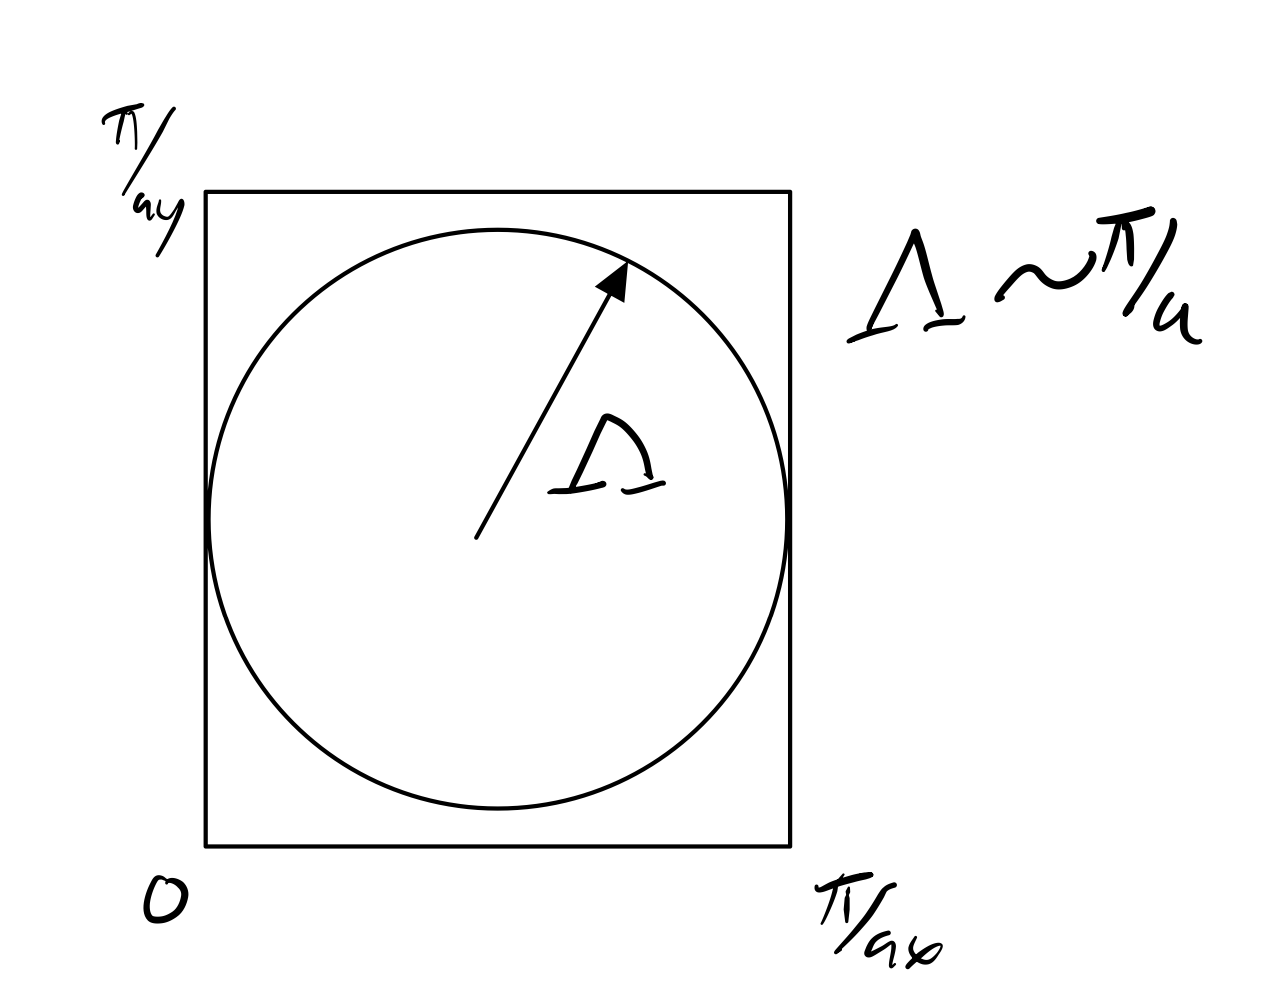
\includegraphics[scale=0.3]{Lectures/Figures/lec8-hypersphere.png}
\end{center}

We rescale the integral by defining $x = q/sqrt{t/k}$ which gives:
\begin{equation}
    F = -\frac{h^2}{2t} + \frac{n\Omega_d}{2}\left(\frac{t}{k}\right)^{d/2}\int_0^{\Lambda/\sqrt{t/k}} dx x^{d-1}\left(\ln t + \ln(1 + x^2 + \frac{Ltx^4}{k^2})\right)
\end{equation}
Note that if $t \ll 1$ the upper limit of the integral goes to infinity. Then we study the integral, and although it looks a little scary, it does turn out to converge. Note that in this limit, $L$ does not matter. It's a bit easier to compute the specific heat than the free energy directly. So, we can take two derivatives of $F$ and find $C$:
\begin{equation}
    C = -\dpd[2]{F}{T} = -n\frac{\Omega_d}{2}\left(\frac{t}{k}\right)^{d/2} \int_0^\infty dx \frac{x^{d-1}}{t^2(1 + x^2 + \frac{Lx^4t}{k^2})^2}
\end{equation} 
For $d > 4$ this is finite.

\subsection{RG approach to Gaussian model}
We return back to the partition function:
\begin{equation}
    Z = \int \mathcal{D}m(\v{q})\exp(-\int_0^\Lambda \frac{d^dq}{(2\pi)^d}\left[\left(\frac{t + kq^2 + Lq^4}{2}\right)\abs{m}^2 + hm(\v{q})\delta(\v{q})\right])
\end{equation}
\subsubsection*{Coarse Grain}
We consider $a < x < ba$ and then consider splitting the momentum space region into $0 < q < \Lambda/b$ and $\Lambda/b < q < \Lambda$, this latter region we call $\sigma(\v{q})$. 

\begin{center}
    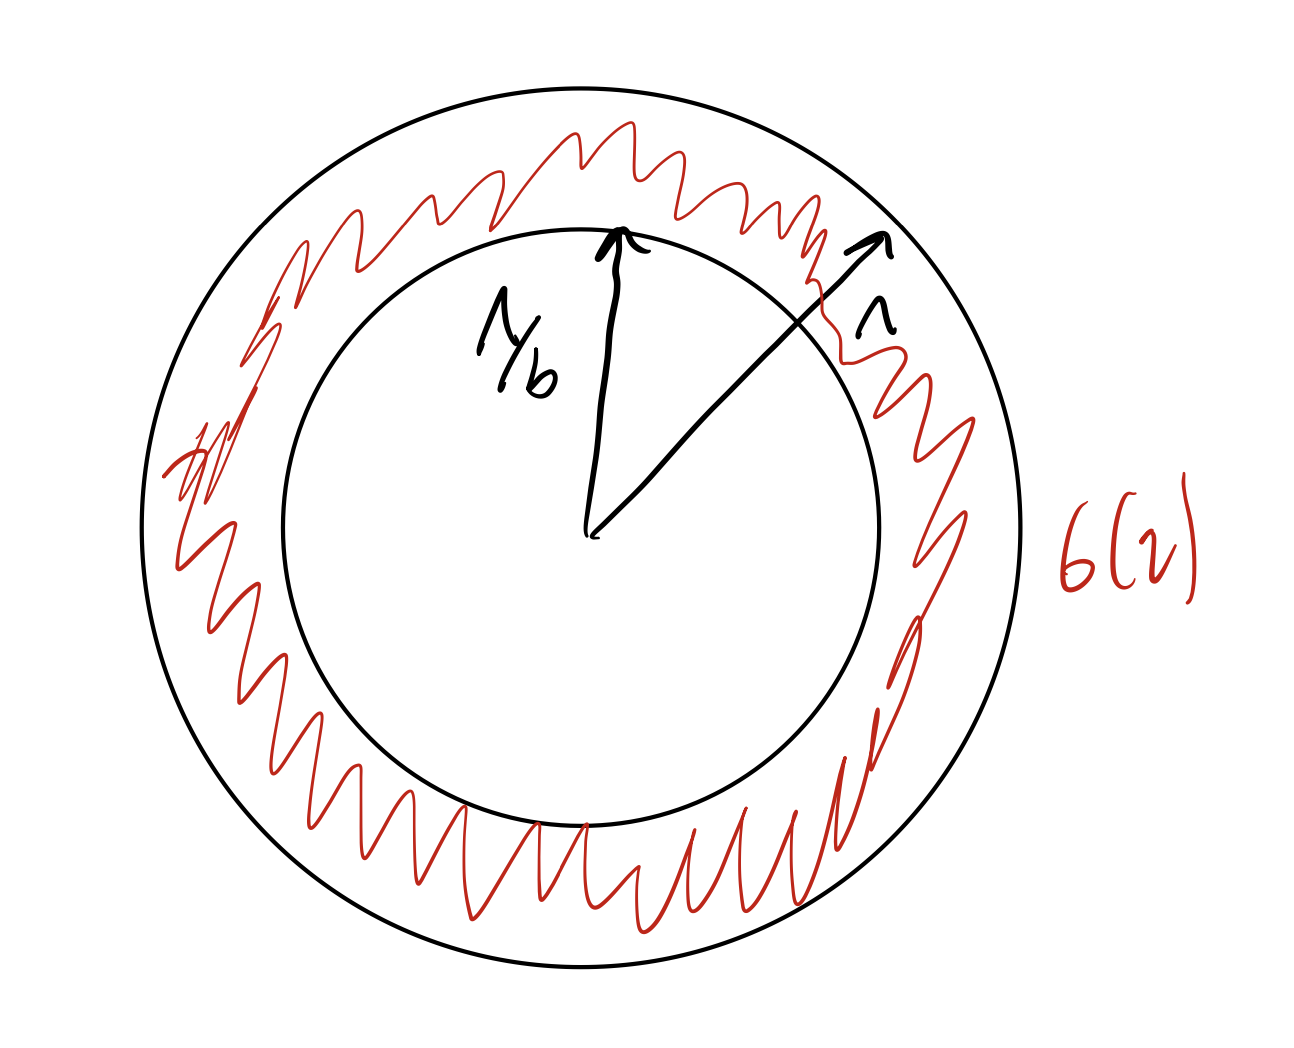
\includegraphics[scale=0.3]{Lectures/Figures/lec8-sphere-split.png}
\end{center}

We then split the integral into two parts:
\begin{equation}
    Z= \exp(-\frac{nV}{2}\int_{\Lambda/b}^\Lambda d^dq \ln(t + kq^2 + Lq^4)) \cdot \int \mathcal{D}m^<(\v{q})\exp(-\int_0^{\Lambda/b}\frac{d^dq}{(2\pi)^d}\left(t + kq^2 + Lq^4\right)\abs{m^<}^2 + hm^<(\v{q})\delta(\v{q}))
\end{equation}
where the first term corresponds to the result of doing the Gaussian integral over $\sigma(\v{q})$. Note we have called the dummy variable of integration $m^<$ to remind ourselves that these are the momenta $< \Lambda/b$ we have not yet integrated over.
\subsubsection*{Rescaling}
Call:
\begin{equation}
    \delta f_b(t) = \frac{n}{2}\int_{\Lambda/b}^\Lambda d^dq \ln(t + kq^2 + Lq^4)
\end{equation}
Now, we rescale $q' = bq$, then:
\begin{equation}
    Z = e^{-V\delta f_b(t)}\int \mathcal{D}m^<(\v{q}')\exp(-\int_0^\Lambda \frac{d^dq'}{(2\pi)^d}b^{-d}\left(\frac{t + kb^{-2}q^2 + Lb^{-4}q'^{4}}{2}\abs{m^<(\v{q}')}^2 + hm^<(\v{q}')\delta(\v{q'})\right))
\end{equation}
where the appropriate dimensional quantities have picked up factors from rescaling.

\subsubsection*{Renormalization}
We now renormalize:
\begin{equation}
    m'(q) = \frac{m^<(q)}{z}
\end{equation}
After we do this, the partition function now becomes:
\begin{equation}
    Z = e^{-V\delta f_b}\int \mathcal{D}m(\v{q})\exp(-\int_0^\Lambda \frac{d^dq}{(2\pi)^d}\left[b^{-d}z^2\left(\frac{t + kb^{-2}q^2 + Lb^{-4}q^4}{2}\right)\abs{m}^2 + zhm(\v{q})\delta(\v{q})\right])
\end{equation}
Nowm we rescale our parameters:
\begin{subequations}
    \begin{align}
        t_{\text{new}} &= z^2b^{-2}t 
        \\ h_{\text{new}} &= z h
        \\ k_{\text{new}} &= z^2b^{-d-2}k 
        \\ L_{new} &= z^2 b^{-d-4}L
    \end{align}
\end{subequations}
The $t = 0, h = 0$ singular point fortunately remain the same with the new parameters. If things are to be scale invariant at the singular/critical point, then $k_{\text{new}} = k$ (since we want the Hamiltonian to transform back to itself at the critical point - we take this as the definition) which enforces:
\begin{equation}
    z = b^{1 + d/2}
\end{equation}
So then:
\begin{equation}
    L_{\text{new}} = b^{-2}L
\end{equation}
so $L$ is irrelevant. (Note: We could not enforce $L_{\text{new}} = L$ and find a consistent set of equations, as if we did, we would find that $k$ would scale to $\infty$. We can propose fixed points, but if we propose $L$ as the leading order variable, then the other variables explode, so it is not a valid fixed point. The trivial scaling dimension of $k$ is $d + 2$ and for $L$ it is $d + 4$). We then find:
\begin{equation}
    t_{\text{neq}} = b^2t
\end{equation}
\begin{equation}
    h_{\text{neq}} = b^{1+d/2}h
\end{equation}
So then:
\begin{equation}
    y_t = 2
\end{equation}
\begin{equation}
    t_n = 1 + d/2
\end{equation}
Which gives us the critical exponents:
\begin{equation}
    \nu = 1/y_t = 1/2
\end{equation}
\begin{equation}
    \Delta = y_n/y_t = \frac{1}{2} + \frac{d}{4}
\end{equation}
\begin{equation}
    \alpha = 2-d\nu = 2 - d/2
\end{equation}
\begin{equation}
    \gamma = 1
\end{equation}
Our fixed point Hamiltonian (which is scale invariant) is:
\begin{equation}
    H^* = \frac{k}{2}\int d^dx \left(\nabla m \right)^2
\end{equation}
our results here agree with the exact solution obtained via solving the Gaussian theory. In the future, we will use the RG to solve problems that are not exactly solvable. But before we go to perturbative RG, a couple of technical points.

\subsection{Scaling dimension}
Consider:
\begin{equation}
    u_n\int d^d x m^n
\end{equation}
If we now find a fixed point and add a perturbation to the model, we can now power count after doing the RG:
\begin{equation}
    u_n\int d^d x m^n \to b^d z^n \int d^dx' m^n
\end{equation}
then, $u_n$ scales as:
\begin{equation}
    u_n' = u_n b^{d+n-nd/2} = u_n b^{y_n}
\end{equation}
and $y_n = n - d\left(\frac{n}{2}-1\right)$. For different $n$:
\begin{subequations}
    \begin{align}
        y_1 &= 1 + d/2
        \\ y_2 &= 2
        \\ y_4 &= 4-d
        \\ y_6 &= 6 - 2d
    \end{align}
\end{subequations}
From $y_4$, we see that the fourth order coefficient is relevant for $d < 4$. From $y_6$, we see that the sixth order term is relevant for $d < 3$. This is then the framework for what we will next when we think about the Wilson-Fisher fixed point, where we include the fourth order coupling. This suggests that there might be a small parameter $\e$ which is the difference in dimensions from $d = 4$; we can't do perturbations in the fields in $d = 3$ (as they grow rapidly); but if we work in dimensions in close to $4$ (i.e. $d = 4 - \e$), then things can be controlled. If we expand in $\e$ and the radius of convergence is $> 1$ then this mathematical trick allows us to obtain results in $d = 3$. This is very close to dimensional regularization in QFT. Historically, a lot of these concepts were already known by Schwinger before they were applied to stat mech, and even before that known to applied mathematicians looking at badly behaved differential equations.